\section{Quasi-Probability Distributions}
Probability distributions in the classical theory of probability are subject to 3 important restrictions, which derive from the Kolmogorov axioms on the system probability measure.
The transition to a quantum theory of probability relaxes one or more of these axioms, and quasi-probability distributions result-these are not necessarily everywhere positive, and regions integrated under such distributions do not in general represent mutually exclusive states as do the analogous regions under true probability distributions.
This corresponds to the relaxation of the first and third of Kolmogorov's axioms.

Several different quasi-probability distribution representations are possible \cite{Walls2008}, and to each is associated a theorem known as the \emph{Optical equivalence theorem} \cite{Sudarshan1963}, for a power series of annihilation and creation operators in a given ordering.
The optical equivalence theorem is concisely stated as follows
\begin{equation}
	\langle g_{\Omega} (\alpha, \alpha^*) \rangle = \langle g_{\Omega} (\hat{a}, \cre) \rangle
\end{equation}
with $g_\Omega$ some power series of $\hat{a}$ and $\cre$, and $\Omega$ the ordering of that power series.
That is to say, the expectation of a power series of the operators $\hat{a}$ and $\cre$ is the same as the expectation value of the same power series with annihilation and creation operators replaced by complex eigenvalues $\alpha$ and $\alpha^*$ respectively, with regard to the appropriate quasiprobability distribution for that operator ordering.
The quasiprobability distributions for each ordering are listed below.

Quasi-probability distributions arise naturally when considering representations of the density operator.
The density operator is in general defined with regards to a complete orthonormal set of projection operators.
However, a diagonal representation of the density operator in terms of an \emph{overcomplete} set of non-orthogonal projectors is also always possible \cite{Sudarshan1963}, and the corresponding representation is in certain systems conceptually and computationally simpler.
The relevant overcomplete set in quantum optics is the set of coherent states of the electromagnetic field defined as the right eigenstates of the annihilation operator
\begin{equation}
\alpha | \alpha \rangle = \ann | \alpha \rangle
\end{equation}
\subsection{Normal Ordering}
An operator ordering is \emph{normal} if in all products of annihilation and creation operators, all creation operators come before annihilation operators \cite{Mandl2010} The Glauber-Sudarshan P function \cite{Cahill1969}:
\begin{equation}
	\dens = \int P(\alpha) | \alpha \rangle \langle \alpha | d^2 \alpha
	\end{equation}
        where $\dd[2]{\alpha} = \dd{Re\{\alpha \}}\dd{Im\{\alpha \}}$, is used for evaluating expectations of normally ordered power series:
\begin{equation}
  \langle \hat{a}^{\dagger n} \hat{a}^{m}  \rangle = \int \alpha^n \alpha^m P (\alpha, \alpha^*) \dd[2]{\alpha}
\end{equation}
P ($\alpha$) does not in general admit an interpretation as a classical probability distribution.
However, the transition between quantum and classical systems is most clearly visible in the P representation; any system with a classical analogue (a coherent state, a chaotic state) has a non-negative, classically interpretable P function, and any with no classical analogue (Fock states, or states exhibiting squeezing, antibunching) will have a P function which is either negative or more singular than delta function.
This statement is not generally true for other quasiprobability distributions \cite{Mandel1995}
\subsubsection{General procedure for evaluating P($\alpha$)}\label{mehta}
There exists a general expression for evaluating the P-function that yields a well-behaved function whenever such a function is possible.
 \cite{Mehta1967}:
\begin{equation}
	P(\alpha) = \frac{1}{\pi^2} \int d^2 \beta \bra{-\beta} \dens \ket{\beta} e^{|\beta|^2} e^{\beta^* \alpha -\alpha^* \beta}
\end{equation}
It is a necessary and suffient condition for this expression for P ($\alpha$) to be standard function that the function $ \bra{\beta} \dens \ket{\beta} e^{|\beta|^2} $ be square integrable.
Should it not be square integrable P ($\alpha$) can only be understood in the context of generalised function theory.
\subsection{Antinormal Ordering}
\emph{Antinormal} ordering is the inverse of normal ordering, in that annihilation operators appear before creation operators.
The associated quasi-probability distribution is the \emph{Husimi-Q Function} \cite{Husimi1940}, defined as the diagonal matrix elements of the density operator in a pure coherent state
\begin{equation}
	Q = \frac{\langle \alpha | \dens | \alpha \rangle}{\pi}
	\label{qdef}
\end{equation}
The Q function is a nonnegative, the density function being a positive operator.
It is also bounded above
\begin{equation}
	Q \leq \frac{1}{\pi}
\end{equation}
Antinormally ordered expectation values can be evaluated as follows:
\begin{equation}
  \langle \hat{a}^n \hat{a}^{\dagger m}  \rangle = \int \alpha^n \alpha^m Q (\alpha, \alpha^*) \dd[2]{\alpha}
\end{equation}
The Q function exists for states which admit no P representation, and unlike the P or W function is always positive.
It does not however always lead to a Fokker-Planck equation with a positive-definite diffusion matrix. 
\subsection{Symmetric Ordering}
The first quasi-probability distribution to be introduced and the most popular in the literature is the \emph{Wigner Function} \cite{Wigner1932} , which satisfies the OET for symmetrically ordered products: those of the form $\frac{\ann \cre + \cre \ann}{2}$
True probability distributions for generalised position and momentum are only possible independently $\rho(x) = |\braket{x}{\psi}|^2$, $\rho(p) = |\braket{p}{\psi}|^2$.
This is fundamental principle of quantum mechanics.
A joint statistical treatment is however available through the Wigner quasi-probability distribution
\begin{equation}
  W(X_1, X_2) = \frac{1}{4 \pi} \int_{-\infty}^\infty \dd{X} e^{\frac{-iXX_2}{2}} \bra{X_1+X} \dens \ket{X_1-X}
\end{equation}
Expressed in terms of the generalised position and momentum in quantum optics: the field quadratures defined $\alpha = X_1 + iX_2$.
Integrating over either quadrature yields the true probability distribution in the other quadrature.
The Wigner function is defined as the \emph{Wigner transform} of the density matrix, a general invertible transformation taking operators to functions on phase space.
Its inverse, the \emph{Weyl transform}, returns functions to operators.
The phase space formulation of quantum mechanics in its original form involves propagating such functions in time using Moyal's Evolution Equation \cite{Curtright2011}.
This same formalism is equivalently applied  through different integral transforms to the other representations.
\subsection{Characteristic Functions}
The above functions are equivalently derived from the antinormal, normal, and symmetric characteristic functions, defined as follows:
\begin{align}
	\chi_{A} (\eta) &= tr\{\dens e^{-\eta^* \hat{a}}e^{\eta \cre } \} \\
	\chi_{N} (\eta) &= tr\{\dens e^{\eta \cre}e^{-\eta^* \hat{a} } \} \\
	\chi_{S} (\eta) &= tr\{\dens e^{\eta^* \hat{a}-\eta \cre } \}
\end{align}
with the corresponding quasiprobability distributions retrieved as the inverse Fourier transform of the corresponding characteristic function
\begin{equation}
 	\{P|Q|W\} = \hat{\mathscr{F}}^{-1} [\chi_{\{N|A|S\}}]
\end{equation}
The existence of the inverse transform is necessary condition for the existence of a particular representation in terms of non-generalised functions.
\subsection{Coherent State Representations}
The form of the density matrix for a system in pure coherent state $ | \alpha_0 \rangle $  is:
\begin{equation}
 	\dens = | \alpha_0 \rangle \langle \alpha_0 |
\end{equation}
\subsubsection{P-function}
From the properties of the delta function, the form of the P-function is evident:
\begin{equation}
	P(\alpha) = \delta^2(\alpha-\alpha_0)
\end{equation}
\subsubsection{Q-function}
The Q-function is evaluated from the definition:
\begin{equation}
	Q(\alpha) = \frac{\langle \alpha | \alpha_0 \rangle \langle \alpha_0 | \alpha \rangle}{\pi} = \frac{{|\langle \alpha | \alpha_0 \rangle |}^2}{\pi} =  \frac{e^{-{|\alpha_0 - \alpha |}^2}}{\pi}
\end{equation}
\subsubsection{Wigner Function}
The Wigner function is recovered from the Wigner transform of $\ket{\alpha_0}\bra{\alpha_0} = \ket{X_1+iX_2}\bra{X_1+iX_2}$
\begin{equation}
	W(x_1, x_2) = \frac{2}{\pi} e^{-\frac{1}{2}[{(x_1-X_1)}^2+{(x_2-X_2)}^2]}
\end{equation}
\begin{figure}[!htb]
  \begin{minipage}{0.5\linewidth}
          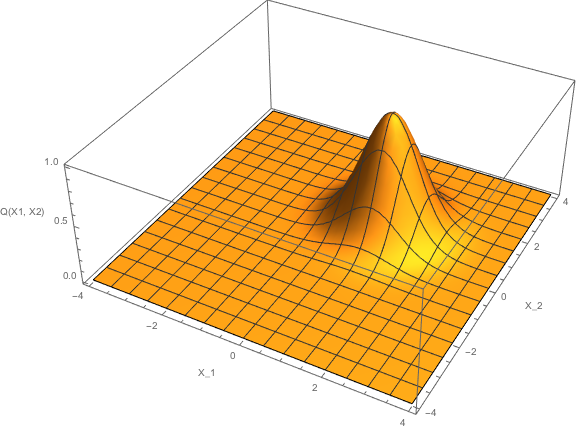
\includegraphics[width=\linewidth]{Q Function-Coherent.png}
	\end{minipage}%
  \begin{minipage}{0.5\linewidth}
          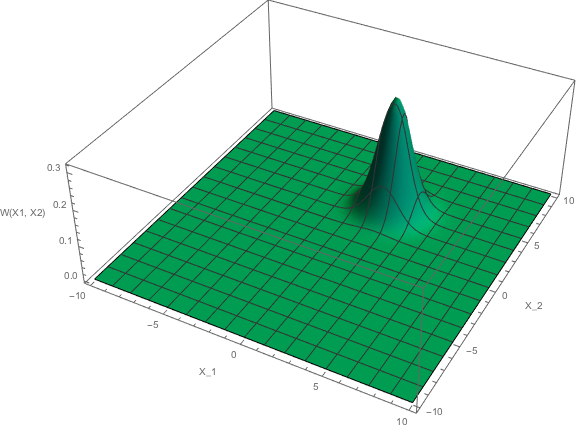
\includegraphics[width=\linewidth]{W Function-Coherent.png}
    \end{minipage}
  \caption{(a) Q function (orange) and Wigner Function (green) for the coherent states $\alpha = 1+i$ and $\alpha = 5+3i$}
\end{figure}
\subsection{Fock state Representations}
\subsubsection{P-function}
Since Fock states have no classical analogue, we would expect the P function associated with the Fock state density matrix $\ket{n}\bra{n}$ should be highly singular or negative.
From \cite{Mehta1967}  P ($\alpha$) is non-singular (not more singular than a $\delta$-function) if and only if $ \bra{\beta} \dens \ket{\beta} e^{|\beta|^2} $ is square integrable.
But, using the Fock state expansion of the coherent states
\begin{align}
	 \bra{\beta} \dens \ket{\beta} e^{|\beta|^2}  &= e^{-|\beta|^2} \sum_{k=0}^\infty \frac {{\beta^*}^k}{k!} \braket{k}{n}\braket{n}{k} \sum_{k=0}^\infty \frac {\beta^k}{k!}e^{|\beta|^2} \\ &= e^{-|\beta|^2} \frac{|\beta|^{2n}}{{n!}^2} e^{|\beta|^2} \\ &= \frac{|\beta|^{2n}}{{n!}^2}
\end{align}
Which is square integrable for no value of n.

A representation in terms of a class of generalised functions called \emph{tempered distributions} is possible\footnote{Specifically, in terms of the derivatives of a Dirac delta function \cite{Gerry2005}}, but the behaviour of such objects makes them difficult to work with.
\subsubsection{Q-function}
Despite the pathological Fock state P-function the Q-function follows simply from the definition
\begin{align}
	 Q(\alpha) = \bra{\alpha} \dens \ket{\alpha}  &= \sum_{k=0}^\infty \frac {{\alpha^*}^k}{k!} \braket{k}{n}\braket{n}{k} \sum_{k=0}^\infty \frac {\alpha^k}{k!}e^{-|\alpha|^2} \\ &= \frac{|\alpha|^{2n}}{{n!}^2} e^{-|\alpha|^2}
\end{align}
\begin{figure}[!htb]
	\begin{minipage}[b]{.5\linewidth}
        \centering \large 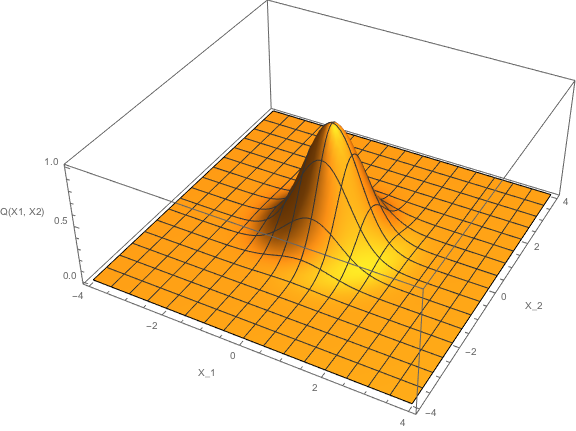
\includegraphics[width=1\linewidth]{Q Function-n=0.png}
	\end{minipage}%
	\begin{minipage}[b]{.5\linewidth}
		\centering\large 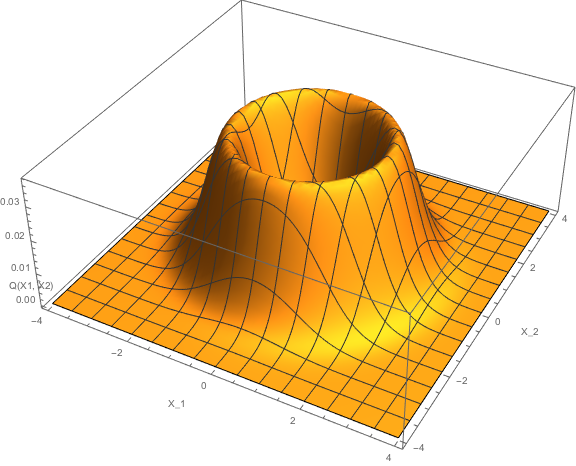
\includegraphics[width = 1\linewidth]{Q Function-n=3.png}
	\end{minipage}
  \caption{Fock State Q Functions for n=0 and n=5}\label{Qfunctions}
\end{figure}
\subsubsection{Wigner function}
The Wigner transform of $\ket{n}\bra{n}$ is \cite[65]{Walls2008}
\begin{equation}
	W(x_1, x_2) = \frac{2}{\pi} {(-1)}^n \mathscr{L}_n(4(x_1^2+x_2^2))e^{-2(x_1^2+x_2^2)}
\end{equation}
Where $\mathscr{L}_n$ is the nth Laguerre Polynomial.
\begin{figure}[!htb]
	\begin{minipage}[b]{.5\linewidth}
		\centering \large 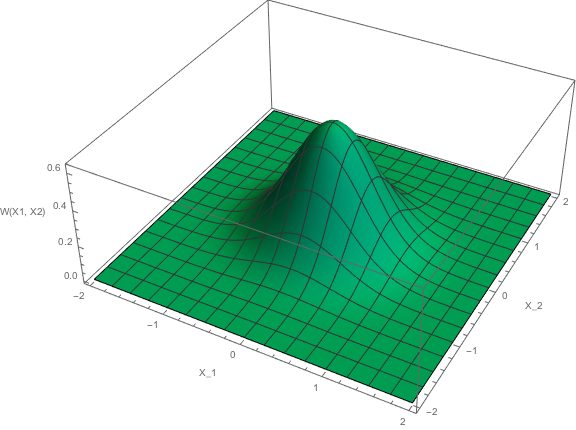
\includegraphics[width=1\linewidth]{W Function-n=0.png}
	\end{minipage}%
	\begin{minipage}[b]{.5\linewidth}
		\centering\large 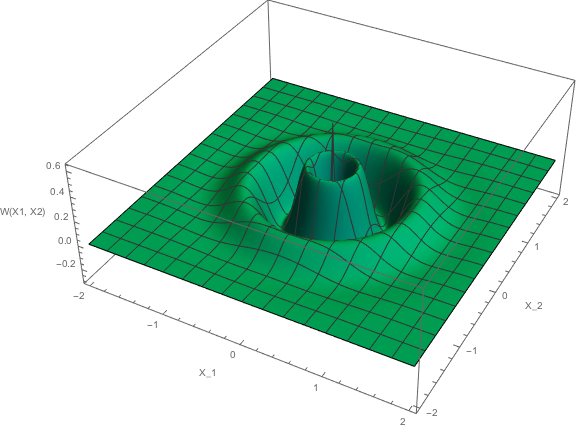
\includegraphics[width = 1\linewidth]{W Function-n=10.png}
	\end{minipage}
	\caption{Fock State Wigner Functions for n=0 and n=10}\label{Wfunctions}
\end{figure}
\subsection{Generalised P Representations}
\label{gen_p}
Any density operator admits a diagonal P representation in terms of distributions, which are computationally and conceptually complicated.
The overcompleteness of the coherent states does not sufficiently restrict the P function, and thus they are not unique.
For this purpose the R representation was proposed \cite{Glauber1963a}. 
This representation does not generally yield positive definite Fokker-Planck diffusion matrices \cite{Walls2008}, and as such it has not seen much use.\\

Introducing an additional complex variable for a coherent basis {$\ket{\beta}_{\beta\in\mathbb{C}}$}, a measure $d\mu(\alpha, \beta)$ and an integration domain $\mathscr{D}\subset\mathbb{C}\times\mathbb{C}$ defines a family of representations of the density matrix, which have had substantial analytical success
 \cite{Drummond1979}.
This formalism is due to \cite{Drummond1980}.
The extension goes 
\begin{equation}
  \dens = \iint_{\alpha, \beta \in \mathscr{D}}P \left( \alpha, \beta \right) \hat{\mathscr{J}} 
  \dd{\mu \left( \alpha, \beta \right)}
          \label{gen_p_rep}
\end{equation}
with
\begin{equation}
  \hat{\mathscr{J}} = \frac{\ket{\alpha}\bra{\beta^*}}{\braket{\beta^*}{\alpha}} 
\end{equation}
We trade a real (quasi-)probability function over a real (classical) phase space, for a (generally) complex function of two complex variables, on a complex phase space.
\subsubsection{Diagonal} 
The measure that recovers the diagonal P representation is
\begin{equation}
  d\mu(\alpha, \beta) = \delta(\alpha-\beta^*)d^2 \alpha d^2 \beta
\end{equation}
$\alpha$ and $\beta = \alpha^*$ now take values on a two-dimensional subset of the complex plane ($\mathbb{C}\times\mathbb{C}$) - the familiar real phase plane.
\subsubsection{Complex}
Letting $\beta, \alpha$ vary independently on two different complex contours $\mathscr{C}, \mathscr{C}'$, and taking as measure
\begin{equation}
  d\mu\left(\alpha, \beta\right) = \dd{\alpha} \dd{\beta}
\end{equation}
The corresponding P function can take complex values.
This representation has been used to derive the photon number distribution of a cavity containing a nonlinear medium \cite{Drummond1979}.
\subsubsection{Positive}
We consider a surface integral over the whole $\alpha$-$\beta$ plane
\begin{equation}
  d \mu(\alpha, \beta) = \dd[2]{\alpha} \dd[2]{\beta}
\end{equation}
In this case the distribution is always positive, and always admits an interpretation as a genuine probability. 
\subsection{Application}
The canonical quantisation of a system consisting of a nonlinear medium inside a cavity leads to a Hamiltonian of the form 
\begin{equation}
  \mathscr{H} = \hbar \delta_{cd} \cre \ann + \hbar \chi \cre{}^ 2 \ann{}^ 2 + \hbar \left( \ann \xi(t) + \cre \xi(t)^* \right) 
\end{equation}
after moving to a rotating frame at the drive frequency.
with $\chi$ a function of the third order anharmonicity of the medium and the electric field mode functions, $\delta_{cd}$ the detuning of the drive from the resonant frequency of the cavity, and $\xi(t)$ the time varying drive envelope \cite{Drummond1979}.
We form a master equation with lindblad dissipators $\mathscr{L}_{\kappa}[\dens]$ and $\mathscr{L}_{\text{therm}}[\dens] = \mathscr{L}_{\bar{n}+1}[\dens] +  \mathscr{L}_{\bar{n}}[\dens]$ representing the dissipation of the cavity field through the mirrors, and interaction with a finite temperature environment with mean photon number $\bar{n}$ respectively.
\begin{equation}
  \dot{\dens} = i\hbar\comm{\ham}{\dens} + \mathscr{L}_{\kappa}[\dens] + \mathscr{L}_{\text{therm}}[\dens]
\end{equation}
We insert the generalised P representation, defined in \cref{gen_p_rep}.
\begin{align}
  \pdv{t} P(\alpha, \beta)  &= \Bigg(\pdv{\alpha} (\kappa \alpha + 2 \chi^* \alpha^2 \beta - \xi(t) )\\ 
                            &- \chi(t) \pdv[2]{\alpha} \alpha^2\\
                            &+ \pdv{\beta} (\kappa^* \beta + 2\chi^* \beta^2 \alpha - \xi^*(t))\\
                            &- \chi^*(t) \pdv[2]{\beta} \beta^2\\
                            &+ (2(\kappa - i\delta_{cd})\bar{n} + \Gamma_E ) \pdv{}{\alpha}{\beta}\Bigg) P(\alpha, \beta)
\end{align}
where we have introduced a term $\Gamma_E$ which accounts for the fluctuation of the drive.

\cite{Haken1975} provides a condition under which exact steady state solutions may be attained. It follows:
For a Fokker-Planck equation of the standard form 
\begin{equation}
  \pdv{t}P(\alpha, \beta) = (\partial_\mu A_\mu (\alpha, \beta) + \frac{1}{2} \partial_\mu \partial_\nu D_{\mu\nu}) P(\alpha, \beta) 
  \label{fokker_planck}
\end{equation}
the potential
\begin{equation}
  V_\rho(\alpha, \beta) = D_{\rho\nu}(\alpha, \beta)^{-1} (2A_\nu(\alpha, \beta) + D_\sigma D_{\nu\sigma}(\alpha, \beta))
\end{equation}
must satisfy
\begin{equation}
  \partial_\mu V_\nu = \partial_\nu V_\mu
\end{equation}
In our case one can verify that the condition is satisfied in the limit $\Gamma = 2(\kappa - i\delta{cd})\bar{n} + \Gamma_E \ll \abs{\chi( \bar{n} + \bar{n}_{\text{cav}} )}$, where $\bar{n}_{\text{cav}}$ is the average photon number in the cavity.

In this limit we can neglect $\Gamma$, the off-diagonal elements of the diffusion matrix for the fokker-planck equation.
The diffusion matrix thus becomes positive-definite, and we have for the drift A and diffusion D
\begin{align}
  A  &= \begin{pmatrix}
  \mqty{(\kappa - i\delta_{cd})\alpha + 2\chi\alpha^2 \beta - \xi(0)\\ (\kappa - i\delta_{cd})\alpha + 2\chi^* \beta^2 \alpha - \xi^*(0)}
       \end{pmatrix}\\
  D  &= \begin{pmatrix}
       \mqty{-2\chi\alpha^2 & 0 \\ 0 & -2 \chi^* \beta^2 }
       \end{pmatrix}
\end{align}
from which the potential condition can be easily verified. 
From here, \cite{Haken1975} gives a prescription for evaluating the P function from the potential
\begin{equation}
  P(\alpha, \beta) = \exp \left( - \int^\alpha \int^\beta \dd{\beta}\dd{\alpha} V_\mu (\alpha, \beta) \right)
\end{equation}
for our parameters, the solution is 
\begin{equation}
  P(\alpha, \beta) = \alpha^{\frac{\kappa-i\delta_{cd}}{\chi}-2} \beta^{{\left[\frac{\kappa-i\delta_{cd}}{\chi}\right]}^*-2}\exp{\frac{\xi(0)}{\chi}\left(\frac{1}{\alpha} + \frac{1}{\beta}\right) + 2\alpha\beta}
\end{equation}
\subsubsection{Moments}
The generalised P function has normal ordered expectation values as its moments, just as the diagonal representation.
On the diagonal integration domain (i.e. $\ket{\alpha} \text{for } \alpha \in \mathbb{C}$) with the diagonal measure setting $\beta = \alpha^*$, there is a term in $\exp{\alpha\beta} = \exp{\abs{\alpha}^2}$ for which the integral on the domain is divergent.
We take instead the complex measure, on two different contours.
The moments of the distribution are the same as the normalisation integral but for the $\alpha$ and $\beta$ exponents.
We take a function with general exponents $c = (\kappa-i\delta_{cd}) / \chi + k $, $d = ((\kappa-i\delta_{cd}) /\chi)^*+q$, where $k, q \in \mathbb{N}$, and make the variable change $\gamma = \flatfrac{1}{\alpha}, \varphi = \flatfrac{1}{\beta}$
\begin{align*}
  P(\gamma, \varphi) &= \gamma^{-c-2} \varphi^{-d-2} \exp{\frac{1}{\gamma\varphi}} \exp{\frac{\xi(0)}{\chi}\left(\gamma + \varphi \right)}\\
                     &= \sum_{n=0}^\infty\flatfrac{\left(\frac{1}{\gamma\varphi}\right)^n}{n!} \times \gamma^{-c-2}\varphi^{-d-2} \exp{\frac{\xi(0)}{\chi}(\gamma+\varphi)}\\
                     &= \sum_{n=0}^\infty\flatfrac{2^n \gamma^{-c-2-n}\varphi^{-d-2-n} \exp{\frac{\xi(0)}{\chi}(\gamma+ \varphi)}}{n!}
\end{align*}
Integrating on contours $\mathscr{C}, \mathscr{C'}$
\begin{align*}
  I(c, d) = \iint_{\mathscr{C}, \mathscr{C}'} \dd{\gamma}\dd{\varphi} P(\gamma, \varphi) &= \sum_{n=0}^\infty\frac{1}{n!} \int_\mathscr{C} \dd{\gamma} \gamma^{-c-n} \exp{\frac{\xi(0)}{\chi}\gamma} \\ 
                                                                                 & \qquad \ \ \times \int_{\mathscr{C}'}\dd{\varphi} \varphi^{-d-n} \exp{\frac{\xi(0)}{\chi}\varphi}
\end{align*}
We take for the contours Hankel paths from $-\infty$ to $-\infty$, anticlockwise, enclosing the origin \cite{Drummond1979}. 
We have then gamma functions as in \cite{TISP}.
\begin{equation}
     \frac{1}{\Gamma(x)} = \left(\frac{t^{1-x}}{2\pi i}\right) \int_{\mathscr{C}} \dd{\eta}\eta^{-x} \exp{\eta x}
\end{equation}
thus
\begin{equation}
  I(c, d) = -4\pi^2 \sum_{n=0}^\infty \frac{2^n \{\flatfrac{\xi(0)}{\chi}\}^{c+d+2(n-1)}}{\Gamma(c+n)\Gamma(d+n)n!}
\end{equation}
using the form of the $_0F_2$ generalized hypergeometric function \cite{Slater1966} \cite{TISP}
\begin{equation}
  _0F_2(c, d, z) = \sum_{n=0}^\infty \left( \frac{ z^n \Gamma(c) \Gamma(d)}{\Gamma(c+n)\Gamma(d+n)n!} \right)
\end{equation}
we have 
\begin{equation}
  I(c, d) = \left( \frac{4\pi^2 \abs{\frac{\xi(0)}{\chi}}^{c+d-2}}{\Gamma(c)\Gamma(d)} \right) {}_0F_2 \left(c, d, 2\abs{\frac{\xi(0)}{\chi}}^2\right)
\end{equation}
Which gives expressions for all normally ordered moments 
\begin{equation}
  \ev{\cre{}^n \ann^m} = \displaystyle \frac{\displaystyle I\left(\frac{\kappa-i\delta_{cd}}{\chi}+n, \frac{\kappa+i\delta_{cd}}{\chi}+m\right)}{\displaystyle I\left(\frac{\kappa-i\delta_{cd}}{\chi}, \frac{\kappa+i\delta_{cd}}{\chi}\right)}
\end{equation}
particularly:
\begin{widetext}
  \begin{align}
    &\text{The cavity field: }\nonumber\\ 
    &\ev{\ann} = \frac{\chi}{\kappa-i\delta_{cd}} \abs{\frac{\xi(0)}{\chi}} {}_0F_2\left(1+ \frac{\kappa-i\delta_{cd}}{\chi}, \frac{\kappa+i\delta_{cd}}{\chi}, 2\abs{\frac{\xi(0)}{\chi}}^2\right) \Bigg/ {}_0F_2 \left(\frac{\kappa-i\delta_{cd}}{\chi}, \frac{\kappa+i\delta_{cd}}{\chi}, 2\abs{\frac{\xi(0)}{\chi}}^2\right)\label{field_duff}\\
    &\text{The 2nd order correlation function: }\nonumber\\
    g^{(2)}(0) =& \frac{\ev{\cre{}^2 \ann{}^2}}{\ev{\cre\ann}^2} =  \cfrac{(\kappa^2 + \delta_{cd}^2){}_0F_2 \left( \frac{\kappa - i \delta_{cd}}{\chi}, \frac{\kappa+i\delta_{cd}}{\chi}, 2\abs{\frac{\xi(0)}{\chi}}^2 \right) {}_0F_2 \left( \frac{\kappa-i\delta_{cd}}{\chi}+2, \frac{\kappa+i\delta_{cd}}{\chi}+2, 2\abs{\frac{\xi(0)}{\chi}}^2 \right)}{(\kappa^2 + \delta_{cd}^2 + 2 \kappa + 1) \left[{}_0F_2\left(\frac{\kappa-i\delta_{cd}}{\chi}+1, \frac{\kappa+i\delta_{cd}}{\chi}+1, 2\abs{\frac{\xi(0)}{\chi}}^2 \right)\right]^2} \label{g2_duff}
  \end{align}
\end{widetext}
From the P function we can also derive the photon statistics, as well as the Wigner function \cite{Kheruntsyan1999}.
